\subsection{Visual proof of correctness}
\label{section:VisualComparison}
To evaluate wether the online implementation produces the same plots with the streaming method as the approach by \textcite{rakuschek2025visual} they are are visually compared on the same input. Each snapshot file is processed on its own with a window size which spans over the entire input. Normally in a streaming scenario significantly smaller windows are chosen due to the reason that they discard older observations and thereby can adapt to non stationary behavior. The result of this is that the covariance matrix represents only the most recent observations instead of the distribution of the whole sequence which would mean that it would become unsuitable to be compared with the offline principal component analysis of the sequence. Additionally the algorithm needs a warm up phase which initially fills the covariance matrix which needs at least window size samples. Recalculating after each window size would mean that the algorithm would not calculate anything just fill its initial buffer. To to circumvent this problem the input data which as explained contains the entire snapshots of all files is to slide this window and thereby to throw out older observations and plot the new status of the fingerprint. Another critical section is the subspace iteration which needs a sufficient number
of updates to converge to a stable solution. With short input sequences, the offline baseline would be
compared against a subspace estimate that has not converged yet.
\\
The time delay embedding uses a time lag of $\tau = 1$ and an embedding dimension of $d = 1500$.
For a fair comparison, the streaming implementation is restarted from scratch for every file,
the same way as the offline version computes each file independently.

\begin{figure}[H]
    \centering
    \begin{adjustwidth}{-2cm}{-2cm}  % je 2cm links und rechts in den Rand hinein
        \centering
        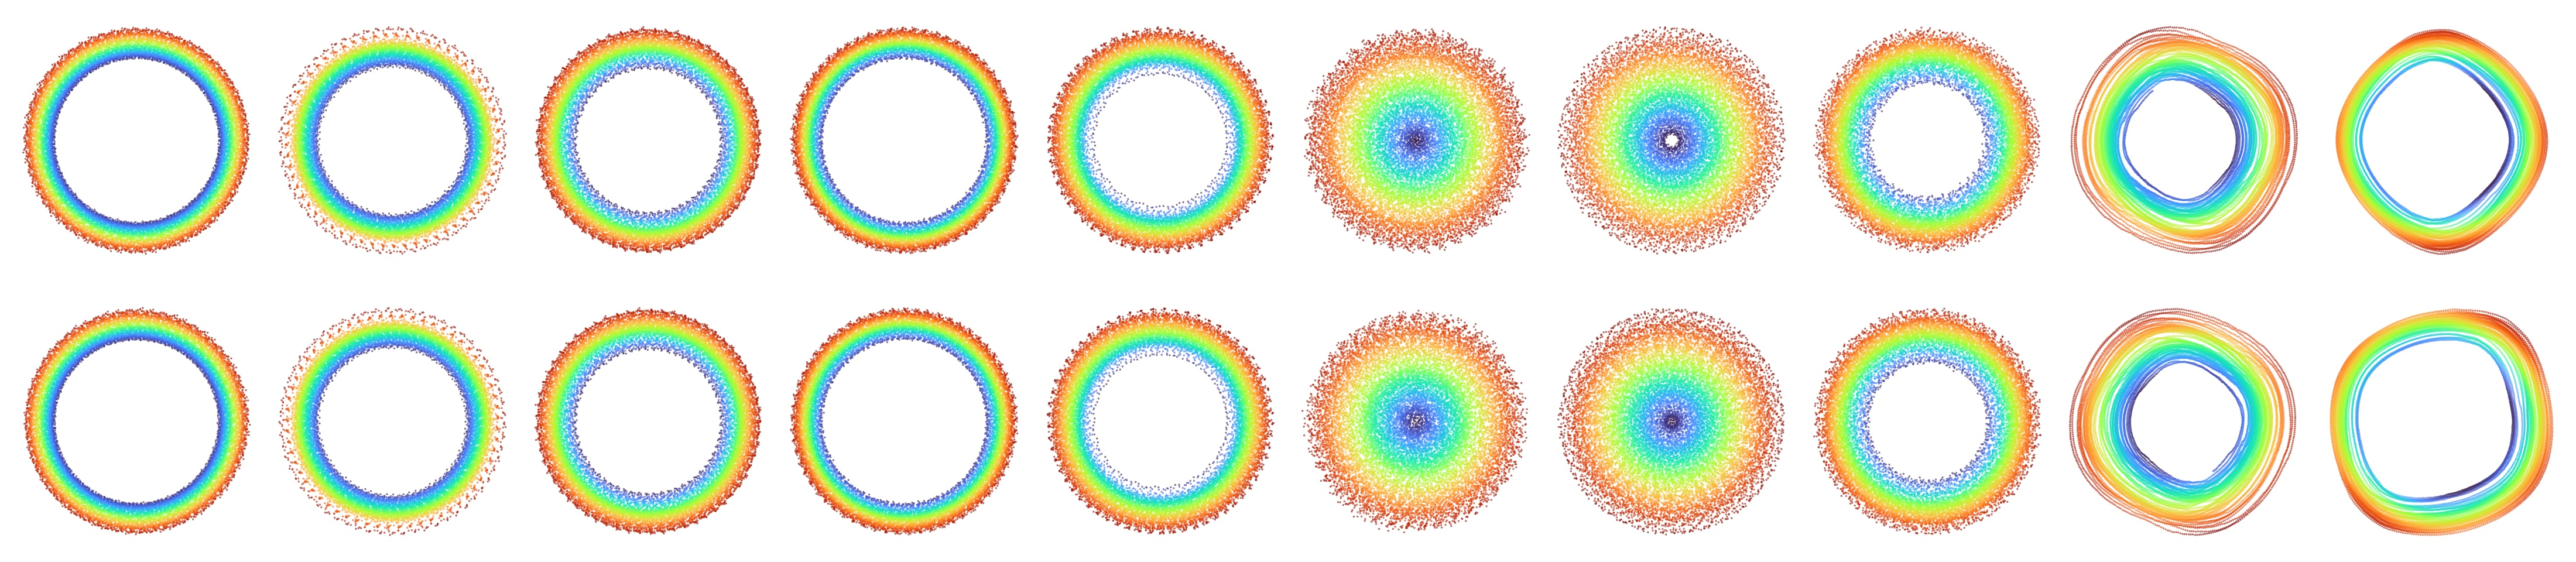
\includegraphics[width=\linewidth]{figures/offlineVsOnlineResults/proof_online_vs_offline.jpg}
    \end{adjustwidth}
    \caption{Fingerprints of the same snapshot files. First row: offline reference. Second row:
    streaming implementation, restarted for every file. }
    \label{fig:offlineVsonline}
\end{figure}

Figure~\ref{fig:offlineVsonline} shows the direct comparison between the offline and the
streaming algorithm. The fingerprints are visually identical, the streaming implementation therefore reproduces the results of the offline approach.